\documentclass[11pt]{article}

\usepackage[final]{acl}
\usepackage{times}
\usepackage{latexsym}
\usepackage[T1]{fontenc}
\usepackage[utf8]{inputenc}
\usepackage{microtype}
\usepackage{graphicx}
\usepackage{booktabs}
\usepackage{amsmath}
\usepackage{xcolor}
\usepackage{url}

% ---------------------------------------------------------------------------
% Every number, table, example and figure in generated/ is produced from the
% notebook outputs by  python analysis/make_report_assets.py results/ report/generated/
% ---------------------------------------------------------------------------
% auto-generated by analysis/make_report_assets.py
\newcommand{\NSST}{150}
\newcommand{\SSTLen}{20.9}
\newcommand{\SSTAccOrig}{91.3}
\newcommand{\SSTBleuOrig}{1.00}
\newcommand{\SSTCosOrig}{1.00}
\newcommand{\SSTChgOrig}{0}
\newcommand{\SSTAccTen}{52.0}
\newcommand{\SSTBleuTen}{0.07}
\newcommand{\SSTCosTen}{0.18}
\newcommand{\SSTChgTen}{64}
\newcommand{\SSTAccTwentyFive}{64.0}
\newcommand{\SSTBleuTwentyFive}{0.10}
\newcommand{\SSTCosTwentyFive}{0.37}
\newcommand{\SSTChgTwentyFive}{62}
\newcommand{\SSTAccFifty}{78.0}
\newcommand{\SSTBleuFifty}{0.16}
\newcommand{\SSTCosFifty}{0.55}
\newcommand{\SSTChgFifty}{59}
\newcommand{\SSTAccHundred}{83.3}
\newcommand{\SSTBleuHundred}{0.19}
\newcommand{\SSTCosHundred}{0.60}
\newcommand{\SSTChgHundred}{57}
\newcommand{\SSTAccTwoFifty}{77.3}
\newcommand{\SSTBleuTwoFifty}{0.19}
\newcommand{\SSTCosTwoFifty}{0.61}
\newcommand{\SSTChgTwoFifty}{56}
\newcommand{\NIMDB}{150}
\newcommand{\IMDBLen}{48.7}
\newcommand{\IMDBAccOrig}{75.3}
\newcommand{\IMDBBleuOrig}{1.00}
\newcommand{\IMDBCosOrig}{1.00}
\newcommand{\IMDBChgOrig}{0}
\newcommand{\IMDBAccTen}{54.7}
\newcommand{\IMDBBleuTen}{0.13}
\newcommand{\IMDBCosTen}{0.18}
\newcommand{\IMDBChgTen}{54}
\newcommand{\IMDBAccTwentyFive}{64.7}
\newcommand{\IMDBBleuTwentyFive}{0.16}
\newcommand{\IMDBCosTwentyFive}{0.41}
\newcommand{\IMDBChgTwentyFive}{51}
\newcommand{\IMDBAccFifty}{69.3}
\newcommand{\IMDBBleuFifty}{0.22}
\newcommand{\IMDBCosFifty}{0.62}
\newcommand{\IMDBChgFifty}{46}
\newcommand{\IMDBAccHundred}{74.0}
\newcommand{\IMDBBleuHundred}{0.25}
\newcommand{\IMDBCosHundred}{0.68}
\newcommand{\IMDBChgHundred}{44}
\newcommand{\IMDBAccTwoFifty}{71.3}
\newcommand{\IMDBBleuTwoFifty}{0.25}
\newcommand{\IMDBCosTwoFifty}{0.69}
\newcommand{\IMDBChgTwoFifty}{43}
\newcommand{\IMDBCutLen}{48}
\newcommand{\FunParsed}{129{,}722}
\newcommand{\FunTag}{38{,}366}
\newcommand{\FunNoAge}{36{,}766}
\newcommand{\FunLen}{36{,}525}
\newcommand{\FunDedup}{36{,}102}
\newcommand{\FunBalanced}{4{,}000}
\newcommand{\AgreeRate}{98.8}
\newcommand{\AgreeN}{994}
\newcommand{\PctTagged}{29.6}
\newcommand{\AgeMedian}{25.5}
\newcommand{\AgeMin}{14}
\newcommand{\AgeMax}{52}
\newcommand{\PctMinor}{4.1}
\newcommand{\NMinor}{165}
\newcommand{\RedditLen}{48.7}
\newcommand{\PctRelationships}{94.3}
\newcommand{\NSubreddits}{10}
\newcommand{\NSubLabels}{2}
\newcommand{\SubLabels}{other, relationships}
\newcommand{\PctOther}{5.7}
\newcommand{\NTest}{200}
\newcommand{\NAdapt}{400}
\newcommand{\NTrain}{3800}
\newcommand{\PronKeep}{102}
\newcommand{\RelKeep}{8}
\newcommand{\PronN}{366}
\newcommand{\RelN}{78}
\newcommand{\PronOrig}{78.0}
\newcommand{\PronTen}{79.1}
\newcommand{\PronTwentyFive}{78.0}
\newcommand{\PronFifty}{78.1}
\newcommand{\PronHundred}{78.0}
\newcommand{\PronTwoFifty}{78.5}
\newcommand{\FSubSOrig}{48.0}
\newcommand{\FSubSTen}{55.0}
\newcommand{\FSubSTwentyFive}{48.3}
\newcommand{\FSubSFifty}{48.2}
\newcommand{\FSubSHundred}{55.0}
\newcommand{\FSubSTwoFifty}{47.9}
\newcommand{\FSubAOrig}{48.3}
\newcommand{\FSubATen}{55.0}
\newcommand{\FSubATwentyFive}{48.2}
\newcommand{\FSubAFifty}{48.3}
\newcommand{\FSubAHundred}{48.3}
\newcommand{\FSubATwoFifty}{48.3}
\newcommand{\FGenSOrig}{83.5}
\newcommand{\FGenSTen}{78.0}
\newcommand{\FGenSTwentyFive}{78.0}
\newcommand{\FGenSFifty}{84.0}
\newcommand{\FGenSHundred}{77.5}
\newcommand{\FGenSTwoFifty}{79.9}
\newcommand{\FGenAOrig}{81.4}
\newcommand{\FGenATen}{78.5}
\newcommand{\FGenATwentyFive}{74.5}
\newcommand{\FGenAFifty}{75.5}
\newcommand{\FGenAHundred}{78.5}
\newcommand{\FGenATwoFifty}{79.0}
\newcommand{\FAgeSOrig}{66.2}
\newcommand{\FAgeSTen}{55.7}
\newcommand{\FAgeSTwentyFive}{57.7}
\newcommand{\FAgeSFifty}{60.1}
\newcommand{\FAgeSHundred}{58.6}
\newcommand{\FAgeSTwoFifty}{59.5}
\newcommand{\FAgeAOrig}{63.8}
\newcommand{\FAgeATen}{58.6}
\newcommand{\FAgeATwentyFive}{56.2}
\newcommand{\FAgeAFifty}{56.9}
\newcommand{\FAgeAHundred}{59.7}
\newcommand{\FAgeATwoFifty}{58.5}
\newcommand{\SubAccOrig}{92.5}
\newcommand{\EnvGPU}{Tesla T4}
\newcommand{\EnvTorch}{2.11.0+cu130}
\newcommand{\EnvTransformers}{5.21.0}
\newcommand{\EnvPython}{3.13.16}
\newcommand{\EnvDpmlm}{1.3.0}
\newcommand{\EnvSbert}{5.7.0}
\newcommand{\EnvSacrebleu}{2.6.0}
\newcommand{\ClipMin}{-3.21}
\newcommand{\ClipMax}{16.30}
\newcommand{\Sensitivity}{19.51}
\newcommand{\JudgeModel}{Qwen/Qwen2.5-3B-Instruct}
\newcommand{\RedBleuTen}{0.17}
\newcommand{\RedCosTen}{0.13}
\newcommand{\RedBleuTwentyFive}{0.20}
\newcommand{\RedCosTwentyFive}{0.39}
\newcommand{\RedBleuFifty}{0.25}
\newcommand{\RedCosFifty}{0.56}
\newcommand{\RedBleuHundred}{0.27}
\newcommand{\RedCosHundred}{0.62}
\newcommand{\RedBleuTwoFifty}{0.28}
\newcommand{\RedCosTwoFifty}{0.66}
\newcommand{\JSstIdenticalM}{5.00}
\newcommand{\JSstIdenticalF}{4.70}
\newcommand{\JSstEpsTenM}{1.00}
\newcommand{\JSstEpsTenF}{1.00}
\newcommand{\JSstEpsFiftyM}{1.25}
\newcommand{\JSstEpsFiftyF}{1.32}
\newcommand{\JSstEpsTwoFiftyM}{1.50}
\newcommand{\JSstEpsTwoFiftyF}{1.60}
\newcommand{\JSstMismatchedM}{1.00}
\newcommand{\JSstMismatchedF}{1.25}
\newcommand{\JRedIdenticalM}{5.00}
\newcommand{\JRedIdenticalF}{3.55}
\newcommand{\JRedEpsTenM}{1.00}
\newcommand{\JRedEpsTenF}{1.00}
\newcommand{\JRedEpsFiftyM}{1.30}
\newcommand{\JRedEpsFiftyF}{1.25}
\newcommand{\JRedEpsTwoFiftyM}{1.48}
\newcommand{\JRedEpsTwoFiftyF}{1.42}
\newcommand{\JRedMismatchedM}{1.02}
\newcommand{\JRedMismatchedF}{1.12}
\newcommand{\NJudge}{40}
\newcommand{\JudgeParse}{100}
\newcommand{\JudgeRho}{0.43}
\newcommand{\JudgeRhoN}{240}
\newcommand{\KappaRegLLMG}{0.47}
\newcommand{\RawRegLLMG}{72}
\newcommand{\KappaRegHumG}{0.90}
\newcommand{\RawRegHumG}{95}
\newcommand{\KappaLLMHumG}{0.42}
\newcommand{\RawLLMHumG}{68}
\newcommand{\KappaRegLLMA}{0.97}
\newcommand{\RawRegLLMA}{99}
\newcommand{\KappaRegHumA}{0.87}
\newcommand{\RawRegHumA}{95}
\newcommand{\KappaLLMHumA}{0.90}
\newcommand{\RawLLMHumA}{96}
\newcommand{\NHuman}{100}
\newcommand{\LLMAttGOrig}{34.0}
\newcommand{\LLMAttAOrig}{32.4}
\newcommand{\LLMAttGTen}{34.7}
\newcommand{\LLMAttATen}{51.3}
\newcommand{\LLMAttGTwentyFive}{28.4}
\newcommand{\LLMAttATwentyFive}{40.9}
\newcommand{\LLMAttGFifty}{31.2}
\newcommand{\LLMAttAFifty}{40.3}
\newcommand{\LLMAttGHundred}{37.3}
\newcommand{\LLMAttAHundred}{35.0}
\newcommand{\LLMAttGTwoFifty}{32.8}
\newcommand{\LLMAttATwoFifty}{35.5}
\newcommand{\NLLMAtt}{100}

\newcommand{\repourl}{\url{https://github.com/bbaatargmq/comp8240-dpmlm-replication}}
\newcommand{\todo}[1]{\textcolor{red}{[#1]}}

\title{Replicating and Extending DP-MLM: Differentially Private Text Rewriting with Masked Language Models on New Review and Self-Disclosure Data}

\author{
  Bayarbaatar Gonchigsuren \\
  Student ID: 48728497 \\
  School of Computing, Macquarie University \\
  \texttt{bayarbaatar.gonchigsuren@students.mq.edu.au}
}

\begin{document}
\maketitle

\begin{abstract}
DP-MLM \citep{meisenbacher-etal-2024-dp-mlm} rewrites text under differential privacy (DP) by masking each content word in turn and sampling its replacement from a clipped, temperature-scaled RoBERTa distribution. We replicate the method with the authors' released package and extend it to two datasets on which it has not been evaluated. On GLUE SST-2, our BLEU and embedding-similarity curves follow the paper's closely at strict budgets and are slightly lower at loose ones, while a static sentiment-utility proxy shows the same trend as the paper's fine-tuning results. Utility carries over to longer IMDb reviews. For privacy, we construct a Reddit dataset of \FunTag{} posts whose authors disclose their gender and age in the title, remove these tags, and attack the rewritten text. Age-bracket inference drops by up to 10 F1 points, but gender inference barely changes. We show that this is because DP-MLM never rewrites stopwords: a classifier that uses only eight third-person pronouns, which refer to the poster's partner, reaches the same gender F1 at every budget. An open LLM used as a judge, validated with control pairs, rates even $\varepsilon=250$ rewrites as poorly meaning-preserving although their embedding similarity is high: DP-MLM keeps a text's topic better than its meaning. All code is public.\footnote{\repourl}
\end{abstract}

% =========================================================================
\section{Introduction}
% =========================================================================
Text often carries personal information that is not confined to fixed fields: a review or a forum post can reveal its author's gender, age or identity through word choice alone. \emph{DP text rewriting} tackles this by replacing a text with a privatised version under a formal differential privacy guarantee \citep{dwork2006differential} before it is shared or used for training. This project replicates \citet{meisenbacher-etal-2024-dp-mlm}, \emph{DP-MLM: Differentially Private Text Rewriting Using Masked Language Models} (Findings of ACL 2024),\footnote{\url{https://aclanthology.org/2024.findings-acl.554/}} one of the unit's default projects. As a default project, we only summarise the method and its evaluation as far as needed to follow the replication.

\paragraph{The method.} Earlier DP rewriting methods paraphrase the input with an autoregressive decoder (DP-Paraphrase, \citealp{mattern-etal-2022-limits}; DP-Prompt, \citealp{utpala2023locally}), which chooses each token without seeing the tokens to its right. DP-MLM instead uses an encoder, RoBERTa-base \citep{liu2019roberta}, which predicts a masked word from both sides of its context. For every non-stopword token, the token is masked, the \emph{original} sentence is concatenated in front of the masked one as extra context, and RoBERTa's logits at the masked position are clipped to $[C_{\min}, C_{\max}]$, so the sensitivity is $\Delta = C_{\max}-C_{\min}$. A replacement is sampled from $\mathrm{softmax}(\text{logits}\cdot\varepsilon/2\Delta)$, which is the exponential mechanism \citep{mcsherry2007mechanism} and is $\varepsilon$-DP per token. A text of $n$ rewritten tokens therefore costs $n\varepsilon$ in total under sequential composition.

\paragraph{Evaluation in the paper.} Utility is measured on GLUE \citep{wang-etal-2018-glue}: a DeBERTaV3-base classifier \citep{he2021debertav3} is fine-tuned on privatised training data and evaluated on original validation data. On four tasks the paper also reports BLEU \citep{papineni-etal-2002-bleu} and Sentence-BERT cosine similarity (CosSim; \citealp{reimers-gurevych-2019-sentence}) between original and rewritten text. Empirical privacy is measured on Trustpilot reviews with author gender \citep{hovy-etal-2015-user} and Yelp reviews from 10 authors \citep{utpala2023locally}, with a \emph{static} attacker (trained on original text) and an \emph{adaptive} attacker (trained on privatised text). Both are summarised by the Relative Gain
\begin{equation}
\mathrm{RG} = \frac{U_r}{U_o} - \frac{P_r}{P_o},
\label{eq:rg}
\end{equation}
where $U$ is utility F1, $P$ is attacker F1, and $o$/$r$ denote original and rewritten text; $\mathrm{RG}>0$ means privacy improved by more than utility was lost. On SST-2, DP-MLM reaches 68.5\% accuracy at $\varepsilon=10$ and 86.1\% at $\varepsilon=250$ against a non-private 95.7\%, ahead of both baselines at strict budgets; on Trustpilot, static gender F1 falls from 69.6 to 59.7 at $\varepsilon=10$ (RG 0.12) and recovers fully by $\varepsilon=100$.

\paragraph{This project.} Section~\ref{sec:replication} replicates the mechanism and its utility evaluation on SST-2. Section~\ref{sec:newdata} introduces the new data: IMDb \citep{maas-etal-2011-learning} and a Reddit self-disclosure dataset we built. Section~\ref{sec:results} reports results on the new data, including an LLM-as-judge evaluation, and Sections~\ref{sec:ethics}--\ref{sec:conclusion} discuss ethics and reflect on the project.

% =========================================================================
\section{Replication of the Original Work}
\label{sec:replication}
% =========================================================================

\subsection{Environment and code}
The authors release their code on GitHub\footnote{\url{https://github.com/sjmeis/DPMLM}} and as the PyPI package \texttt{dpmlm}. All experiments ran in Google Colab notebooks (\texttt{dp\_mlm\_replication.ipynb} and \texttt{llm\_evaluation.ipynb}) on an \EnvGPU{} GPU with Python \EnvPython, PyTorch \EnvTorch, Transformers \EnvTransformers, \texttt{dpmlm} \EnvDpmlm, sentence-transformers \EnvSbert{} and sacreBLEU \EnvSacrebleu{} \citep{post-2018-call}. Each notebook runs end to end with \emph{Runtime $\rightarrow$ Run all} (about 45 and 15 minutes); a script in \texttt{analysis/} turns their outputs into the tables of this report, so no number was copied by hand. Data samples use seed 42; DP sampling is itself random, so individual rewrites differ between runs.

Getting the official code to run required two fixes, both caused by library drift rather than by the method. First, recent NLTK versions need the \texttt{punkt\_tab} resource, which the package does not download. Second, \texttt{dpmlm} 1.3.0 sets \texttt{torch.backends.cuda.matmul.}\allowbreak\texttt{fp32\_precision} at import time, an attribute that only exists in very recent PyTorch releases, so the import fails on Colab. The notebook wraps this one line in \texttt{try}/\texttt{except} before importing the package.

\paragraph{An instructive first attempt.} Before using the package we re-implemented the mechanism from the paper's description (\texttt{early\_attempt/} in the repository). That version differed from the paper in five ways: (i)~logits were clipped to hand-picked bounds ($\pm5$ or $\pm10$) instead of bounds calibrated on RoBERTa logits; (ii)~the temperature was $(C_{\max}-C_{\min})/\varepsilon$, missing the factor~2 of the exponential mechanism, so the real guarantee was $2\varepsilon$; (iii)~only one token or a random three-token span was rewritten, not every content word; (iv)~one script omitted the concatenation of the original sentence; and (v)~similarity was TF-IDF cosine rather than sentence embeddings. Its outputs looked plausible but its numbers were not comparable with the paper. The lesson is that the paper's description is correct, but the details that determine the privacy guarantee (calibration and temperature) are easy to get wrong, and the released code is the real specification.

\paragraph{Mechanism settings.} We use the package defaults, which follow the paper: RoBERTa-base, English stopwords and punctuation left unchanged, the original sentence concatenated as context, and clipping bounds $[C_{\min}, C_{\max}] = [\ClipMin, \ClipMax]$, i.e.\ $\Delta = \Sensitivity$. The paper derives the bounds as $(\mu, \mu+4\sigma)$ of RoBERTa logits on 1{,}000 SST-2 sentences but does not print them, so we could only check that the package bounds follow this rule. We use the batched rewriting function, which predicts all masked positions of a text in parallel with the same per-token mechanism.

\subsection{Evaluation protocol}
We privatise \NSST{} randomly sampled SST-2 validation sentences \citep{socher-etal-2013-recursive} (mean length \SSTLen{} words) at each of the paper's five budgets and compute corpus BLEU (sacreBLEU, reported on a 0--1 scale as in the paper), mean CosSim with \texttt{all-MiniLM-L6-v2} (the embedding model family of the paper), and the share of original words not kept in an alignment of original and rewrite (``\% changed''). For sentiment utility we did not repeat the paper's protocol of fine-tuning DeBERTaV3 three times per privatised training set: privatising the 67k SST-2 training sentences is roughly 3.4M masked predictions per budget, beyond our Colab budget. We report instead a \emph{static utility proxy}: the accuracy of an off-the-shelf DistilBERT SST-2 classifier on the rewritten validation sentences. It measures whether a standard model still reads the right sentiment after rewriting. It should follow the paper's trend but be lower, because a classifier fine-tuned on privatised text learns to read the noise and a fixed one cannot.

\begin{table*}[t]
\centering
\small
\begin{tabular}{llrrrrrr}
\toprule
 & & Orig. & $\varepsilon$=10 & 25 & 50 & 100 & 250 \\
\midrule
BLEU & paper & -- & 0.08 & 0.11 & 0.19 & 0.22 & 0.23 \\
 & ours & 1.00 & 0.07 & 0.10 & 0.16 & 0.19 & 0.19 \\
CosSim & paper & -- & 0.17 & 0.37 & 0.61 & 0.65 & 0.67 \\
 & ours & 1.00 & 0.18 & 0.37 & 0.55 & 0.60 & 0.61 \\
Acc (\%) & paper$^\dagger$ & 95.7 & 68.5 & 76.5 & 84.1 & 86.2 & 86.0 \\
 & ours$^\ddagger$ & 91.3 & 52.0 & 64.0 & 78.0 & 83.3 & 77.3 \\
\% changed & ours & 0 & 64 & 62 & 59 & 57 & 56 \\
\bottomrule
\end{tabular}

\caption{Replication on SST-2 ($n=\NSST$). \textit{Paper}: DP-MLM results from \citet[Tables 1--2]{meisenbacher-etal-2024-dp-mlm}. $^\dagger$DeBERTaV3 fine-tuned on privatised training data, mean of 3 runs. $^\ddagger$Off-the-shelf DistilBERT SST-2 classifier on privatised validation sentences (static proxy). ``\% changed'': share of original words not kept (word alignment).}
\label{tab:sst2}
\end{table*}

\begin{table}[t]
\centering
\small
\begin{tabular}{@{}p{0.16\linewidth}p{0.77\linewidth}@{}}
\toprule
Original & The food was cold and the waiter was rude, so we are never coming back. \\
\midrule
$\varepsilon$=10 & The novelty was glass and the breakout was embattled, so we are even damn class. \\
$\varepsilon$=25 & The start was cold and the waiter was ignorant, so we are ever come back. \\
$\varepsilon$=50 & The lunch was poor and the server was bad, so we are never starting return. \\
$\varepsilon$=100 & The dinner was frozen and the waitress was friendly, so we are never travelling back. \\
$\varepsilon$=250 & The food was colder and the waiter was mean, so we are still going through. \\
\bottomrule
\end{tabular}

\caption{DP-MLM rewrites of one sentence at each budget (single random draw from our notebook).}
\label{tab:demo}
\end{table}

\subsection{Results}
Table~\ref{tab:sst2} compares our numbers with the paper and Table~\ref{tab:demo} shows example rewrites. The lexical and semantic curves are reproduced closely at strict budgets: at $\varepsilon=10$ and 25 our BLEU (\SSTBleuTen, \SSTBleuTwentyFive) and CosSim (\SSTCosTen, \SSTCosTwentyFive) are within 0.01 of the paper. The shape of the curve is also the same: most of the gain happens between $\varepsilon=25$ and 50, and utility saturates after $\varepsilon=100$ (paper: BLEU 0.22$\rightarrow$0.23; ours \SSTBleuHundred$\rightarrow$\SSTBleuTwoFifty). At loose budgets our values are lower, by up to 0.04 BLEU and 0.06 CosSim at $\varepsilon=250$.

The static accuracy proxy rises from \SSTAccTen\% at $\varepsilon=10$ to \SSTAccHundred\% at $\varepsilon=100$, against \SSTAccOrig\% on original text. Relative to its own non-private value, the proxy keeps 57\% of the baseline accuracy at $\varepsilon=10$ and 91\% at $\varepsilon=100$; the paper's fine-tuned classifier keeps 72\% and 90\%. As expected, the proxy is lower than the paper's fine-tuned accuracy at strict budgets (\SSTAccTen{} vs.\ 68.5 at $\varepsilon=10$) and close to it at $\varepsilon=100$ (\SSTAccHundred{} vs.\ 86.2). The dip at $\varepsilon=250$ (\SSTAccTwoFifty\%) is within noise: with 150 sentences the standard error of an accuracy near 80\% is about 3.3 points, and each budget is a single random draw.

Three factors can explain the remaining gap at high $\varepsilon$. First, SST-2 sentences are lower-cased and pre-tokenised (\emph{``it 's''}, \emph{`` , ''}) while DP-MLM outputs detokenised text, so even unchanged words can count as BLEU mismatches; BLEU also depends on its implementation and tokenisation \citep{post-2018-call}, which the paper does not specify. Second, we use the current package (1.3.0, with batched prediction and a sliding context window added in 2025) rather than the code version of the paper. Third, our sample is \NSST{} sentences rather than the full validation set. A notable observation is that even at $\varepsilon=250$ about half of the words are changed (\SSTChgTwoFifty\%); many replacements are close synonyms or inflections (\emph{waiter}$\rightarrow$\emph{server}, \emph{lives}$\rightarrow$\emph{live}), which is why CosSim stays high while BLEU stays low. We consider the replication of the mechanism and its lexical/semantic utility curves successful, and the replication of downstream utility partial.

\paragraph{What was not replicated.} We did not rerun the Trustpilot and Yelp privacy experiments or the DP-Paraphrase/DP-Prompt baselines. The paper's Trustpilot sample and Yelp author split are not released with the code, DP-Paraphrase needs a separately distributed fine-tuned GPT-2, and each baseline multiplies GPU time. Instead, we apply the paper's privacy protocol, with both attacker types and RG, to our constructed dataset (Section~\ref{sec:results}), which tests the same claim on new data.

% =========================================================================
\section{Construction of New Data}
\label{sec:newdata}
% =========================================================================
We use one existing dataset that DP-MLM has not been evaluated on, to test utility on longer text, and one constructed dataset, to test privacy in the way Trustpilot and Yelp do in the paper.

\subsection{Existing data: IMDb movie reviews}
IMDb \citep{maas-etal-2011-learning}\footnote{\url{https://huggingface.co/datasets/stanfordnlp/imdb}} contains 50{,}000 movie reviews with balanced binary sentiment labels. It is close to SST-2 in task but different in form: reviews are long (about 230 words), informal, written in natural casing and contain HTML line breaks. Length matters for DP-MLM, because the total budget grows as $n\varepsilon$ and runtime grows linearly with $n$. We sample \NIMDB{} test reviews, remove \texttt{<br />} tags and keep the leading sentences up to 60 words (mean \IMDBLen{} words). The non-private baseline is measured on the same truncated text. Evaluation is identical to SST-2.

\subsection{Constructed data: Reddit self-disclosure}
\paragraph{Motivation.} Trustpilot and Yelp test whether rewriting hides \emph{who} wrote a text. We wanted a dataset where (a)~the sensitive attribute is something the authors disclosed about themselves, not inferred by researchers; (b)~there is more than one sensitive attribute; and (c)~the domain is personal narrative, where privatisation matters most.

\paragraph{Source.} We use the Reddit TL;DR corpus \citep{volske-etal-2017-tl} in the filtered version of \citet{stiennon2020learning}, distributed on HuggingFace as \texttt{trl-lib/tldr}.\footnote{\url{https://huggingface.co/datasets/trl-lib/tldr}} Each example has a subreddit, a title and a post. In advice subreddits, posters conventionally tag themselves in the title, e.g.\ \emph{``Me [24 F] with my boyfriend [27 M] of 2 years\ldots''}. These tags give labels without annotation cost.

\paragraph{Pipeline.} The construction is fully scripted (Part 4 of the notebook):
\begin{enumerate}
\setlength\itemsep{0pt}
\item \textbf{Collect:} parse subreddit, title and post of every example.
\item \textbf{Extract labels:} a regular expression keeps posts whose title \emph{starts} with the poster's own tag (\emph{Me [24F]}, \emph{I (31 m)}, \emph{(f/22)}, \ldots). This is the main difficulty: titles also tag partners and family members (\emph{``my bf [27 M]''}), and only the first-person tag identifies the poster. Labels are gender (M/F) and age bracket ($\le$25 vs.\ $>$25, close to the median age).
\item \textbf{Remove leakage:} delete every age/gender tag from the post, drop posts that still state the poster's age in words (\emph{``I'm 24''}, \emph{``24 years old''}), replace URLs and \texttt{u/} usernames with placeholders, and replace person names found by spaCy NER with \texttt{[NAME]}. Indirect cues (\emph{boyfriend}, \emph{college}) are kept on purpose: they are the realistic signal that privatisation has to remove.
\item \textbf{Filter:} keep posts of 15--60 words after cleaning (to bound DP cost) and remove duplicates.
\item \textbf{Sample:} draw 4{,}000 posts balanced over gender $\times$ age bracket. The utility label is the subreddit, with subreddits below 5\% of the sample merged into \emph{other}.
\end{enumerate}

\begin{table}[t]
\centering
\small
\begin{tabular}{lr}
\toprule
Step & Posts \\
\midrule
posts parsed & 129{,}722 \\
poster tag in title & 38{,}366 \\
no explicit age in body & 36{,}766 \\
15-60 words & 36{,}525 \\
deduplicated & 36{,}102 \\
balanced sample & 4{,}000 \\
\bottomrule
\end{tabular}

\caption{Construction funnel of the Reddit self-disclosure dataset.}
\label{tab:funnel}
\end{table}

\begin{table*}[t]
\centering
\small
\begin{tabular}{@{}p{0.15\linewidth}p{0.81\linewidth}@{}}
\toprule
\textbf{F, $<$=25} \newline r/dating\_advice & Hi, it's my first time writing here - also english is not my native language, so please excuse any mistakes. My problem is that I realized I can't cope with rejection. \\
\midrule
\textbf{F, $>$25} \newline r/relationships & I haven't been in a serious relationship since I was 22 and that lasted 5 years. It was a mutual break up since we grew apart and wanted different things. \\
\midrule
\textbf{M, $<$=25} \newline r/relationships & Hi, what's up guys. Thanks for all the help Reddit is sick. So, 8 months ago my first love broke up with me. Just to say, I was a wreck. \\
\midrule
\textbf{M, $>$25} \newline r/relationships & My girlfriend and I recently moved to a new town where we have a limited circle of friends but both enjoy being active and social so we are hoping to meet new people. \\
\bottomrule
\end{tabular}

\caption{Snippets from the constructed dataset after cleaning (one per gender $\times$ age-bracket cell). The tags were removed from the text; the bold labels were mined from the title.}
\label{tab:reddit-ex}
\end{table*}

\paragraph{Statistics.} Table~\ref{tab:funnel} shows the construction funnel and Table~\ref{tab:reddit-ex} shows example data. \PctTagged\% of the \FunParsed{} posts carry a first-person tag in the title, and very few are lost to the leakage and length filters, leaving \FunDedup{} posts. In the balanced sample, ages range from \AgeMin{} to \AgeMax{} (median \AgeMedian) and posts have \RedditLen{} words on average. The tagging convention is specific to relationship forums, so \PctRelationships\% of the sample comes from r/relationships; the utility label therefore has only \NSubLabels{} classes (\SubLabels) with \PctOther\% in \emph{other}, which turned out to matter (Section~\ref{sec:privacy}). We split the sample into \NTest{} test posts and \NTrain{} training posts, of which \NAdapt{} are also privatised at every budget for the adaptive attacker. Figure~\ref{fig:reddit-overview} (appendix) shows the age and subreddit distributions.

\paragraph{Label quality and agreement.} Labels come from the posters' own words, so the main risk is an \emph{extraction} error (e.g.\ picking up the partner's tag), not disagreement about the attribute. We checked labels in three ways. (1)~\emph{Internal consistency:} where the post body repeats a first-person tag, it agrees with the title label (age within one year, same gender) in \AgreeRate\% of \AgreeN{} cases. (2)~\emph{LLM annotator:} an instruction-tuned LLM (\JudgeModel) read the title and post of a random audit sample of 100 extracted posts and stated the poster's gender and age (prompt in Appendix~\ref{app:prompts}); Table~\ref{tab:agreement} reports Cohen's $\kappa$ \citep{cohen1960coefficient} against the regex labels. (3)~\emph{Manual check of disagreements:} we read the title of every post on which the two disagreed.

Agreement on age bracket is almost perfect ($\kappa=\KappaRegLLMA$; the only disagreement is a ``?'' answer). Agreement on gender is only moderate ($\kappa=\KappaRegLLMG$, \RawRegLLMG\% raw agreement), but the confusion is entirely one-sided: all 28 disagreements are posts labelled \emph{M} by the regex for which the LLM answered \emph{F}, and in every case the title states a male poster (e.g.\ \emph{``I [m20] am getting bored of my [f20] girlfriend''}). Often the LLM appears to copy the partner's tag, but it also answers \emph{F} for titles with no female tag at all (\emph{``Me (23m) with my friends (22m)''}), which indicates a systematic bias of the 3B model rather than ambiguity in the data. We therefore found no extraction error in the audit sample, and the moderate $\kappa$ measures the weakness of the LLM annotator, not of the labels. A full independent human annotation of the sample was planned but not completed in time; it would be the first addition to this dataset.

\begin{table}[t]
\centering
\small
\begin{tabular}{llrrr}
\toprule
Attribute & Pair & $n$ & $\kappa$ & Agree (\%) \\
\midrule
gender & regex vs LLM & 100 & 0.47 & 72 \\
gender & regex vs human & 100 & 0.90 & 95 \\
gender & LLM vs human & 100 & 0.42 & 68 \\
age bracket & regex vs LLM & 100 & 0.97 & 99 \\
age bracket & regex vs human & 100 & 0.87 & 95 \\
age bracket & LLM vs human & 100 & 0.90 & 96 \\
\bottomrule
\end{tabular}

\caption{Label agreement on the 100-post audit sample. ``Regex'': labels mined from titles. ``?'' answers count as disagreement.}
\label{tab:agreement}
\end{table}

% =========================================================================
\section{Results on New Data}
\label{sec:results}
% =========================================================================

\subsection{Utility on IMDb}
\begin{table}[t]
\centering
\small
\setlength{\tabcolsep}{3.5pt}
\begin{tabular}{llrrrrrr}
\toprule
 & & Orig. & 10 & 25 & 50 & 100 & 250 \\
\midrule
BLEU & SST-2 & 1.00 & 0.07 & 0.10 & 0.16 & 0.19 & 0.19 \\
 & IMDb & 1.00 & 0.13 & 0.16 & 0.22 & 0.25 & 0.25 \\
CosSim & SST-2 & 1.00 & 0.18 & 0.37 & 0.55 & 0.60 & 0.61 \\
 & IMDb & 1.00 & 0.18 & 0.41 & 0.62 & 0.68 & 0.69 \\
Acc (\%) & SST-2 & 91.3 & 52.0 & 64.0 & 78.0 & 83.3 & 77.3 \\
 & IMDb & 75.3 & 54.7 & 64.7 & 69.3 & 74.0 & 71.3 \\
\% chg. & SST-2 & 0 & 64 & 62 & 59 & 57 & 56 \\
 & IMDb & 0 & 54 & 51 & 46 & 44 & 43 \\
\bottomrule
\end{tabular}

\caption{Utility on SST-2 (replication) and IMDb (new) by budget $\varepsilon$; IMDb reviews truncated to $\le$60 words. Acc is the static sentiment proxy.}
\label{tab:imdb}
\end{table}

Table~\ref{tab:imdb} and Figure~\ref{fig:utility} compare IMDb with SST-2. IMDb follows the same monotone curve and the same saturation after $\varepsilon=100$, so the paper's utility behaviour generalises to longer, informal reviews. Lexical overlap is clearly higher on IMDb (BLEU \IMDBBleuTen--\IMDBBleuTwoFifty{} vs.\ \SSTBleuTen--\SSTBleuTwoFifty) and fewer words are changed (\IMDBChgTwoFifty\% vs.\ \SSTChgTwoFifty\% at $\varepsilon=250$). We attribute this mainly to tokenisation, since IMDb is not pre-tokenised, and to a higher share of stopwords in conversational text. Sentiment is also better preserved relative to the non-private value: \IMDBAccHundred\% vs.\ \IMDBAccOrig\% at $\varepsilon=100$ (98\% of the baseline, against 91\% on SST-2), plausibly because a 50-word review repeats its sentiment several times and some of these cues survive. The non-private accuracy on truncated IMDb (\IMDBAccOrig\%) is lower than on SST-2 because the opening sentences of a review often do not yet contain the verdict. Utility per token is thus similar or better on longer text, but the guarantee is not: an IMDb text of \IMDBLen{} words consumes several times the total budget of an SST-2 sentence. The paper mentions the $n\varepsilon$ composition, but its benchmark of short sentences does not expose this.

\begin{figure*}[t]
\centering
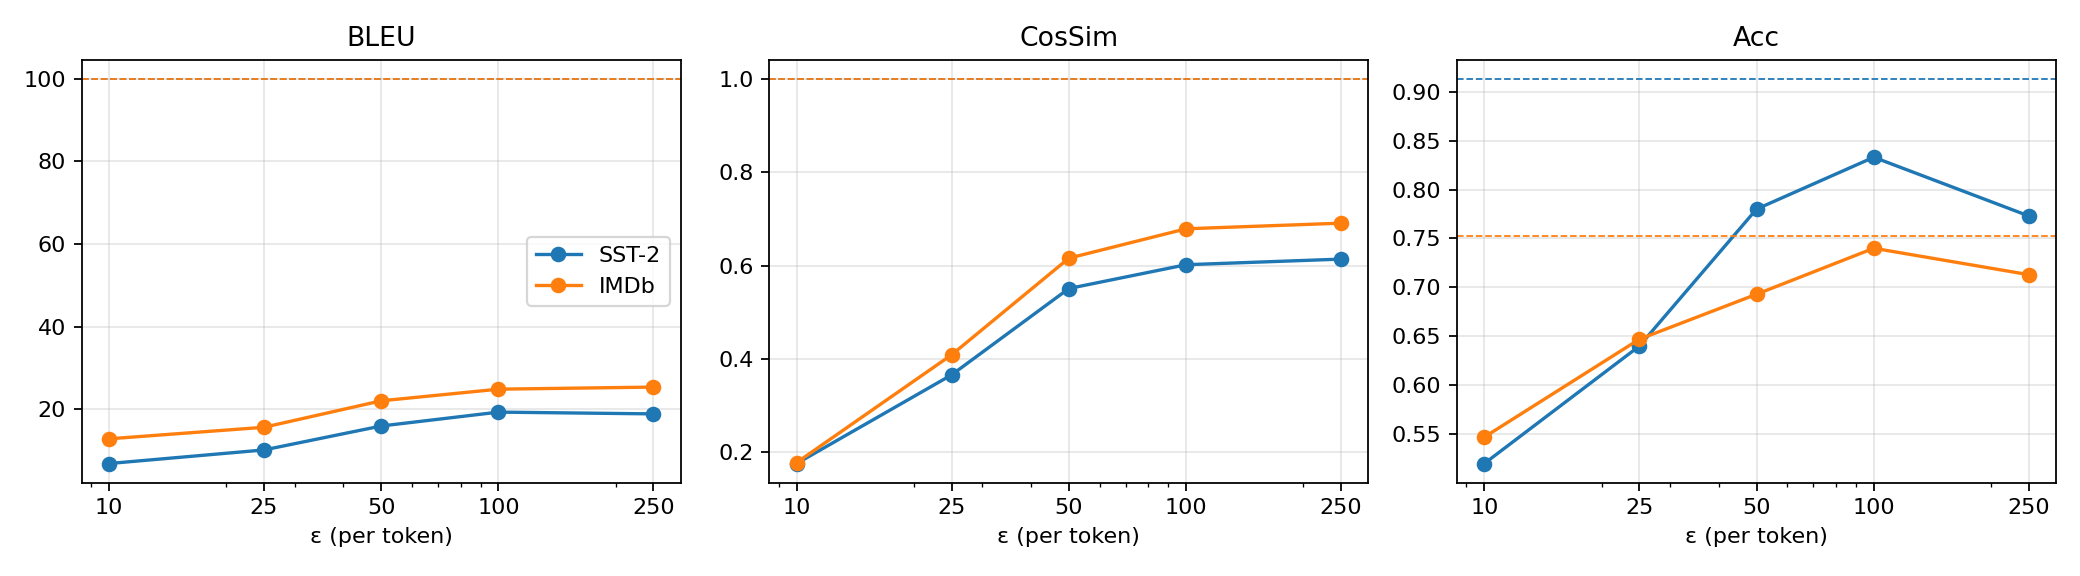
\includegraphics[width=\textwidth]{generated/utility_sst2_imdb.png}
\caption{BLEU, CosSim and static sentiment accuracy against $\varepsilon$ (log scale) for SST-2 and IMDb. Dashed lines: non-private values.}
\label{fig:utility}
\end{figure*}

\subsection{Privacy on the Reddit self-disclosure data}
\label{sec:privacy}
We follow the paper's protocol with lighter models. The utility task is subreddit classification and the privacy tasks are gender and age-bracket inference, all with TF-IDF (1--2-grams) and logistic regression as a fast stand-in for DeBERTaV3. The \emph{static} attacker is trained on original text and tested on privatised test posts; the \emph{adaptive} attacker is trained on \NAdapt{} privatised training posts at the same $\varepsilon$ (its ``Orig.'' column uses the same posts unprivatised). We also ran a zero-shot LLM attacker on 100 test posts. Table~\ref{tab:reddit} gives macro-F1 and RG; chance level is 50 for both attributes.

\begin{table*}[t]
\centering
\small
\begin{tabular}{llrrrrrr}
\toprule
Task & Attacker & Orig. & 10 & 25 & 50 & 100 & 250 \\
\midrule
Subreddit & static & 48.0 & 55.0 & 48.3 & 48.2 & 55.0 & 47.9 \\
 & adaptive & 48.3 & 55.0 & 48.2 & 48.3 & 48.3 & 48.3 \\
\midrule
Gender & static & 83.5 & 78.0 & 78.0 & 84.0 & 77.5 & 79.9 \\
 & adaptive & 81.4 & 78.5 & 74.5 & 75.5 & 78.5 & 79.0 \\
 & pronouns only & 78.0 & 79.1 & 78.0 & 78.1 & 78.0 & 78.5 \\
 & LLM zero-shot & 34.0 & 34.7 & 28.4 & 31.2 & 37.3 & 32.8 \\
\midrule
Age bracket & static & 66.2 & 55.7 & 57.7 & 60.1 & 58.6 & 59.5 \\
 & adaptive & 63.8 & 58.6 & 56.2 & 56.9 & 59.7 & 58.5 \\
 & LLM zero-shot & 32.4 & 51.3 & 40.9 & 40.3 & 35.0 & 35.5 \\
\midrule
RG gender & static & -- & 0.21 & 0.07 & -0.00 & 0.22 & 0.04 \\
RG age bracket & static & -- & 0.30 & 0.13 & 0.09 & 0.26 & 0.10 \\
RG gender & adaptive & -- & 0.17 & 0.08 & 0.07 & 0.04 & 0.03 \\
RG age bracket & adaptive & -- & 0.22 & 0.12 & 0.11 & 0.06 & 0.08 \\
\bottomrule
\end{tabular}

\caption{Results on the constructed Reddit dataset (macro-F1 \%, $n_{\text{test}}=\NTest$). Lower attacker F1 means better privacy. ``Pronouns only'': logistic regression on counts of eight third-person pronouns (\emph{he, him, his, himself, she, her, hers, herself}) trained on original text. The utility task is degenerate (always predicts the majority subreddit), so RG here reflects only the privacy term; see text.}
\label{tab:reddit}
\end{table*}

\paragraph{Utility task.} The subreddit classifier predicts \emph{relationships} for almost every post: its accuracy is \SubAccOrig\%, the majority rate, and its macro-F1 (\FSubSOrig) is that of a majority classifier on two classes. Its F1 moves only when one or two \emph{other} posts happen to be classified correctly (\FSubSTen{} at $\varepsilon=10$). The utility term in RG is therefore flat and uninformative, and the positive RG values in Table~\ref{tab:reddit} reflect only the drop in attacker F1. This is a weakness of our dataset design, discussed in Section~\ref{sec:conclusion}; we use the BLEU/CosSim of the rewrites and the LLM judge (Section~\ref{sec:judge}) as utility evidence for Reddit instead.

\paragraph{Age.} On original text, the static attacker infers the age bracket with \FAgeSOrig{} F1, so age is leaked, if weakly. Rewriting reduces this to \FAgeSTen{} at $\varepsilon=10$ and to about 58--60 at all larger budgets; the adaptive attacker behaves similarly (\FAgeAOrig$\rightarrow$\FAgeATen). The effect is real but modest and almost independent of $\varepsilon$, which is consistent with DP-MLM changing about half of the words even at $\varepsilon=250$.

\paragraph{Gender.} Gender is strongly leaked (static \FGenSOrig{} F1 on original text) and DP-MLM barely hides it: static F1 is \FGenSTen{} at $\varepsilon=10$ and between 77 and 84 at other budgets, and the adaptive attacker is similar. This is a much weaker effect than the paper's Trustpilot result, where static gender F1 fell by 10 points at $\varepsilon=10$. We traced the cause to the stopword rule of DP-MLM. In heterosexual relationship posts, the poster's partner is referred to with \emph{he} or \emph{she}, and these pronouns are English stopwords that DP-MLM never rewrites. In the test posts, the count of third-person pronouns after rewriting at $\varepsilon=10$ is essentially unchanged (\PronN{} occurrences before rewriting, \PronKeep\% of that number after), while only \RelKeep\% of explicit relationship nouns (\emph{boyfriend, wife, \ldots}) survive. A classifier that sees \emph{only} eight pronoun counts reaches \PronOrig{} F1 on original text and \PronTen--\PronTwoFifty{} on rewritten text at every budget, i.e.\ it explains almost all of the remaining gender leakage. Table~\ref{tab:demo-nurse} in the appendix shows the effect on our demo sentence. This is a new, concrete failure mode: the formal guarantee covers only the tokens that are rewritten, and the choice of which tokens are ``safe'' to keep is a privacy decision in itself.

\paragraph{LLM attacker and RG.} The zero-shot LLM attacker failed: on \emph{original} text it reaches only \LLMAttGOrig{} (gender) and \LLMAttAOrig{} (age) macro-F1, below the chance level of 50, and its scores on rewritten text (\LLMAttGTen{} and \LLMAttATen{} at $\varepsilon=10$) are in the same range. Such F1 values come from near-constant predictions, consistent with the bias seen in the annotator role. The LLM row therefore says nothing about DP-MLM and is not used in our conclusions; a larger or better-prompted model would be needed for a meaningful LLM adversary. RG is positive at every budget (largest at $\varepsilon=10$: 0.21 for gender and 0.30 for age, static), but given the flat utility term this only restates the privacy result. With $n=200$ test posts, the standard error of an F1 near 60--80 is about 3 points, so the non-monotone variation between $\varepsilon \ge 25$ is mostly noise.

\begin{figure*}[t]
\centering
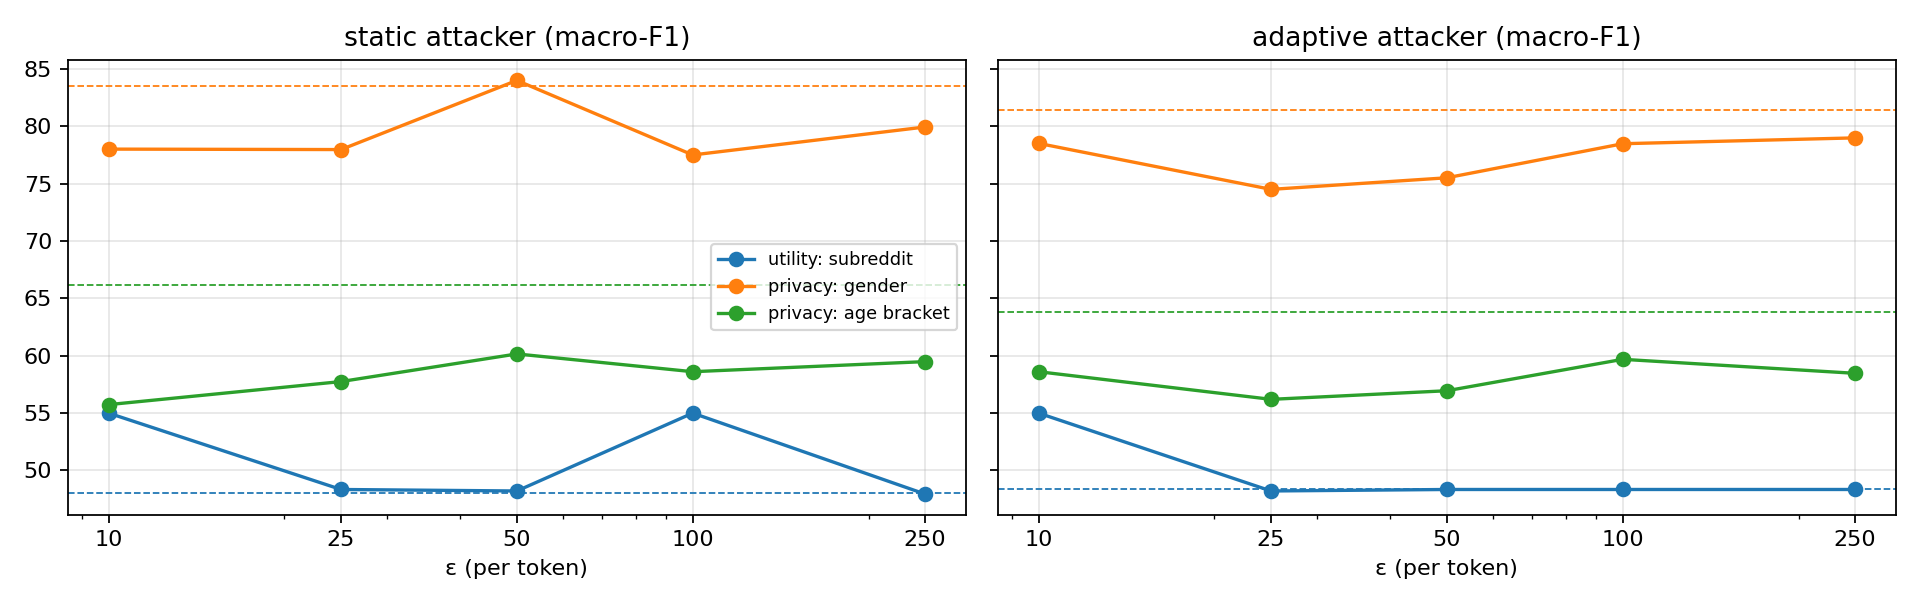
\includegraphics[width=\textwidth]{generated/reddit_privacy_utility.png}
\caption{Macro-F1 of the utility model and the two TF-IDF attackers on the Reddit data. Dashed lines: values on original text.}
\label{fig:privacy}
\end{figure*}

\subsection{LLM-as-judge}
\label{sec:judge}
BLEU measures surface overlap and CosSim embedding closeness, but neither says whether a rewrite is readable English or whether a person would consider the meaning kept. Following the LLM-as-judge paradigm \citep{zheng2023judging}, we give \JudgeModel{} (greedy decoding) an (original, rewrite) pair and ask for two 1--5 ratings, \emph{meaning preservation} and \emph{fluency} (prompt in Appendix~\ref{app:prompts}). We judge \NJudge{} SST-2 sentences and \NJudge{} Reddit test posts at $\varepsilon \in \{10, 50, 250\}$. To check the judge we add two controls per text: an \emph{identical} pair (should score 5/5) and a \emph{mismatched} pair, in which the rewrite is replaced by a different text from the same dataset (meaning should be $\approx$1 while fluency stays high). \JudgeParse\% of answers followed the format. For reference, the Reddit rewrites have BLEU/CosSim of \RedBleuTen/\RedCosTen{} at $\varepsilon=10$ and \RedBleuTwoFifty/\RedCosTwoFifty{} at $\varepsilon=250$.

\begin{table}[t]
\centering
\small
\resizebox{\columnwidth}{!}{\begin{tabular}{llrrr}
\toprule
Data & Condition & Meaning & Fluency & CosSim \\
\midrule
SST-2 & identical (control) & 5.00 & 4.70 & 1.00 \\
 & $\varepsilon$=10 & 1.00 & 1.00 & 0.18 \\
 & $\varepsilon$=50 & 1.25 & 1.32 & 0.57 \\
 & $\varepsilon$=250 & 1.50 & 1.60 & 0.63 \\
 & mismatched (control) & 1.00 & 1.25 & 0.20 \\
\midrule
Reddit & identical (control) & 5.00 & 3.55 & 1.00 \\
 & $\varepsilon$=10 & 1.00 & 1.00 & 0.14 \\
 & $\varepsilon$=50 & 1.30 & 1.25 & 0.58 \\
 & $\varepsilon$=250 & 1.48 & 1.42 & 0.68 \\
 & mismatched (control) & 1.02 & 1.12 & 0.23 \\
\bottomrule
\end{tabular}
}
\caption{Mean LLM-judge ratings (1--5) and mean CosSim per condition. Controls: identical text and an unrelated text.}
\label{tab:judge}
\end{table}

Table~\ref{tab:judge} gives the results. On the rewrites, the judge's meaning score has a Spearman correlation of $\rho=\JudgeRho$ with CosSim ($n=\JudgeRhoN$). The \emph{meaning} scale passes both controls: identical pairs receive \JSstIdenticalM{} on both datasets and mismatched pairs \JSstMismatchedM{} (SST-2) and \JRedMismatchedM{} (Reddit). The \emph{fluency} scale does not: mismatched pairs consist of fluent human-written text, yet they receive only \JSstMismatchedF{} and \JRedMismatchedF, so the 3B judge does not rate fluency independently of meaning, and we do not interpret its fluency scores further. On the rewrites, the judge is far harsher than CosSim. Every rewrite at $\varepsilon=10$ gets the minimum meaning score, and even at $\varepsilon=250$ the mean is only \JSstEpsTwoFiftyM{} (SST-2) and \JRedEpsTwoFiftyM{} (Reddit), while CosSim is above 0.6. Reading the rewrites supports the judge: at $\varepsilon=250$, \emph{``engrossing and moving in its own right''} becomes \emph{``interactive and walking in its own manner''} and \emph{``deserves to be considered as a possible successor''} becomes \emph{``loves to be rejected as a proper response''}. These sentences share topic words with the original, which embedding similarity rewards, but their meaning is changed or reversed. SST-2 and Reddit are judged alike. The judge thus adds a finding that the automatic metrics hide: DP-MLM rewrites at the paper's budgets keep the \emph{topic} of a text much better than its \emph{propositional meaning}. The judge complements but does not replace human evaluation: it is a small open model, its fluency scale failed our control, its ratings were not validated against human ratings, and LLM judges are known to prefer fluent text \citep{zheng2023judging}. In our evaluation the LLM has three roles: a quality judge (this section), a second annotator of the constructed labels (Table~\ref{tab:agreement}) and a zero-shot attacker (Table~\ref{tab:reddit}).

\subsection{Comparison with the replication}
The utility side of DP-MLM generalises well by the paper's own metrics: IMDb reproduces the SST-2 curves, with sentiment better preserved on longer text. The LLM judge qualifies this for both the original and the new data: what is preserved is mostly topic and sentiment polarity, not the specific meaning of the sentence. The privacy side is more mixed than in the paper. On Trustpilot, rewriting at $\varepsilon=10$ removed about 14\% of the attacker's F1 (69.6$\rightarrow$59.7); on our data it removes 16\% for age (\FAgeSOrig$\rightarrow$\FAgeSTen) but only 7\% for gender (\FGenSOrig$\rightarrow$\FGenSTen), and the gender result is explained by tokens the mechanism leaves untouched by design. Benchmarks such as Trustpilot, where gender is mostly expressed through content words, can therefore overstate the protection DP-MLM gives in personal narratives.

% =========================================================================
\section{Ethical Considerations}
\label{sec:ethics}
% =========================================================================
\paragraph{In the original paper.} The paper's ethics statement argues that no harm was done because all datasets were public, and notes that Yelp uses pseudonymous user IDs. Three issues deserve more discussion. First, the privacy experiments \emph{train attackers} that infer gender and identify authors; such classifiers are dual-use, even when built only to measure protection. Second, Trustpilot gender is a binary label taken from user profiles and collected for sociolinguistic research; reusing it for privacy attacks is allowed by its licence but is not the purpose for which it was collected. Third, and most important for users of the method, the guarantee is per token: a text of $n$ tokens has a total budget of $n\varepsilon$, so at the ``strict'' $\varepsilon=10$ a 20-token sentence has $\varepsilon=200$, which gives little formal protection. Our gender result adds that untouched stopwords are outside the guarantee altogether. The authors say that DP-MLM protects privacy ``empirically and by proxy'', but a practitioner who reads only the per-token $\varepsilon$ could overestimate the protection, and an easy-to-install package increases this risk.

\paragraph{If we published on the new data.} The Australian Code for the Responsible Conduct of Research \citep{nhmrc2018code} asks researchers to act with honesty, rigour, transparency, fairness, respect and accountability, and to obtain ethics approval where required. Research on data about people, even public data, is human research under the National Statement \citep{nhmrc2023national}. Publishing on our Reddit dataset would raise the following issues.
\begin{itemize}
\setlength\itemsep{0pt}
\item \textbf{Ethics review and consent.} Reddit users did not consent to their age and gender being used as labels for profiling experiments, and many social media users do not expect their posts to be used in research \citep{fiesler2018participant}. The work would probably qualify for low-risk review with a waiver of consent (public data, consent impracticable), but this requires approval by a Human Research Ethics Committee \emph{before} publication; this coursework project was not submitted for review.
\item \textbf{Minors.} Our regular expression accepts ages from 13, and \NMinor{} posts (\PctMinor\%) in our sample are by posters who state an age under 18. Research involving children needs additional protection under the National Statement, so a published version should exclude these posts (a one-line filter in the notebook).
\item \textbf{Re-identification.} Reddit posts are searchable, so a verbatim quote can be traced to an account even after tags and names are removed. We show only short cleaned snippets here and would release post IDs and code rather than texts with attribute labels attached.
\item \textbf{Respect and fairness.} The tagging convention reduces gender to M/F, so non-binary posters are excluded, and the population (English-speaking users of relationship forums) is not representative. Our pronoun finding also depends on mostly heterosexual relationships; results should not be generalised beyond this sample.
\item \textbf{Dual use.} The age and gender attackers, including the zero-shot LLM attacker, are profiling tools. They are needed to evaluate privatisation, but we would not release trained attackers.
\item \textbf{Licence and terms.} The TL;DR corpus is released for research, but its content remains subject to Reddit's terms of use.
\item \textbf{Transparency of AI use.} Generative AI was used to help write code and text; all outputs were checked and the author is responsible for them, in line with the Code's principle of accountability.
\end{itemize}

% =========================================================================
\section{Conclusions and Reflections}
\label{sec:conclusion}
% =========================================================================
\paragraph{Replication.} The core of DP-MLM was easy to replicate with the released package once two library-version problems were fixed. The BLEU and CosSim curves on SST-2 match the paper within 0.01 at $\varepsilon \le 25$ and are slightly lower at loose budgets, and the sentiment proxy shows the paper's trend. Re-implementing the method from the paper alone was much harder: the calibrated clipping bounds are not printed and the factor~2 in the temperature is easy to miss, and both change the guarantee. The full downstream protocol (DeBERTaV3 fine-tuning on privatised GLUE, three seeds, nine tasks) is expensive because every training token must be rewritten, which makes it the least reproducible part of the paper on student compute.

\paragraph{Generalisation.} Utility generalised: IMDb behaves like SST-2. Privacy generalised only partly: age leakage is reduced by up to 10 F1 points, while gender leakage stays high because DP-MLM keeps pronouns. This shows that a privatisation method should be evaluated on data where the sensitive attribute is expressed in different ways, not only through content words.

\paragraph{What we would do differently.} (1)~\emph{Choose the utility task before the data.} Our subreddit label was degenerate because self-tagging is a convention of one forum; a better utility task would be, for example, relationship type or the post's TL;DR summary scored by similarity. (2)~Measure the pronoun effect directly by also running DP-MLM with stopword replacement enabled, which the package supports. (3)~Use DeBERTaV3 for utility and attackers so that numbers are directly comparable with the paper, and repeat runs to reduce noise. (4)~Complete an independent human annotation of the audit sample and validate the LLM judge against human ratings; a larger judge model is needed, since our 3B model failed the fluency control and was biased as an annotator and attacker. (5)~Plan compute around the $n\varepsilon$ and $O(n)$ costs from the start; truncating texts to 60 words was a pragmatic choice that changes the task. Finally, label extraction was easier than expected, but checking for indirect leakage was harder, and the difficulty of a privacy benchmark depends on cleaning choices that the original datasets do not document either.

\section*{Limitations}
Our samples are small (\NSST{} SST-2 sentences, \NIMDB{} IMDb reviews, \NTest{} Reddit test posts) and each configuration was run once, so differences of a few points are within noise. The sentiment accuracy is a static proxy rather than the paper's fine-tuning protocol, attackers are TF-IDF models rather than DeBERTaV3, and the LLM judge, annotator and attacker is a 3B-parameter open model.

\bibliography{references}

\appendix
\section{Additional figures and examples}
\label{app:figs}

\begin{figure*}[t]
\centering
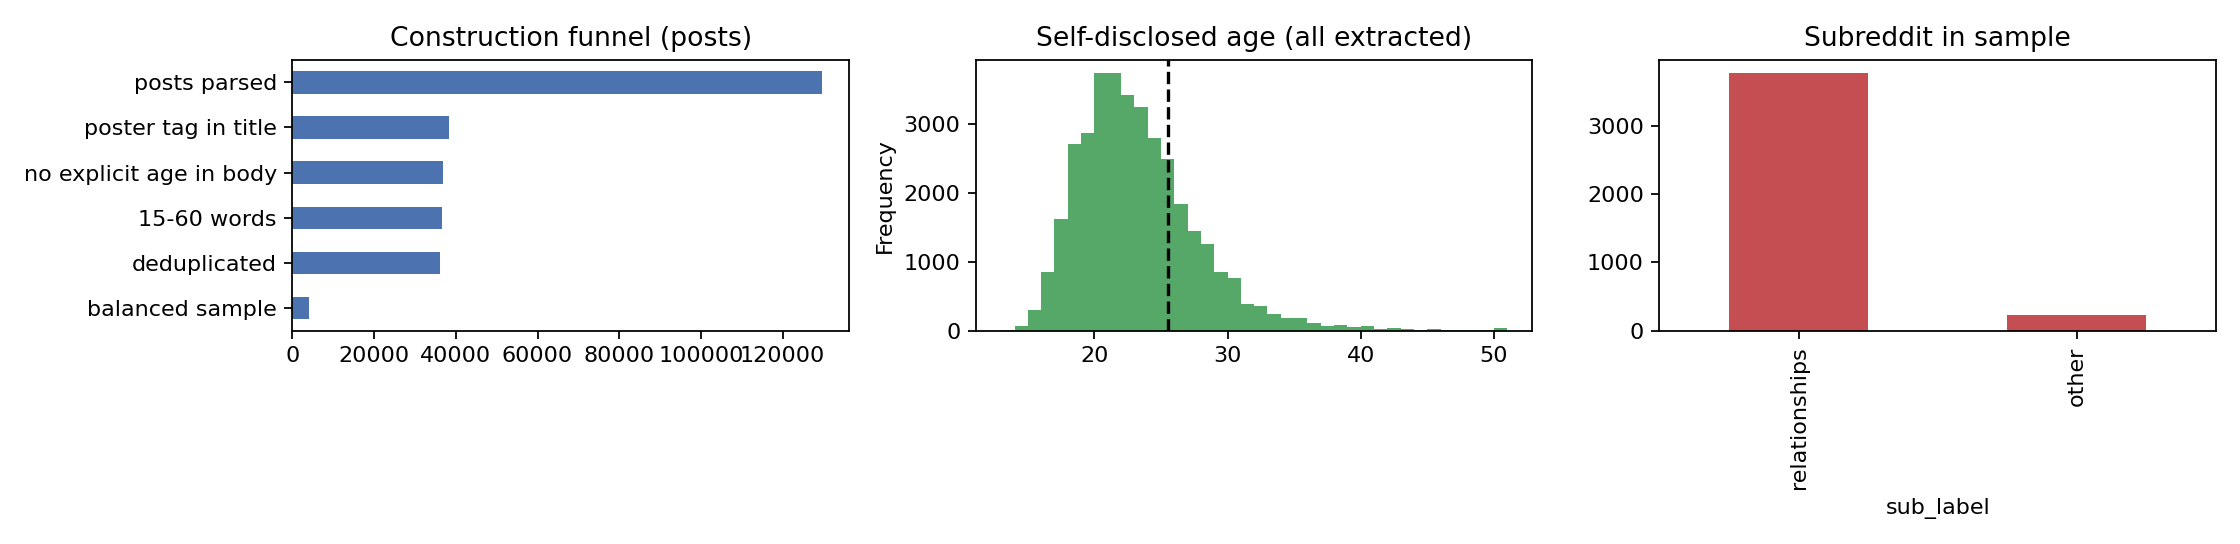
\includegraphics[width=\textwidth]{generated/reddit_dataset_overview.png}
\caption{Reddit self-disclosure dataset: construction funnel, self-disclosed ages (dashed line: bracket boundary), and subreddits in the experiment sample.}
\label{fig:reddit-overview}
\end{figure*}

\begin{table}[h]
\centering
\small
\begin{tabular}{@{}p{0.16\linewidth}p{0.77\linewidth}@{}}
\toprule
Original & I am a 24 year old nurse and my boyfriend is a high school teacher. \\
\midrule
$\varepsilon$=10 & I am a vend suffering tom lung and my pregnant is a coroner violence brush. \\
$\varepsilon$=25 & I am a 20 yea oldest professor and my it is a ok grade clerk. \\
$\varepsilon$=50 & I am a 32 year o nurse and my fiance is a secondary school driver. \\
$\varepsilon$=100 & I am a 21 month iron nurse and my hobby is a high school instructor. \\
$\varepsilon$=250 & I am a 24 year elderly nurse and my girlfriend is a high school teachers. \\
\bottomrule
\end{tabular}

\caption{Demo sentence with self-disclosure. Stopwords (\emph{I, am, my, is, a}) never change; the age (24) survives at $\varepsilon=250$, while the partner noun is replaced (\emph{fiance}, \emph{girlfriend}).}
\label{tab:demo-nurse}
\end{table}

\begin{table}[h]
\centering
\small
\begin{tabular}{@{}p{0.16\linewidth}p{0.77\linewidth}@{}}
\toprule
Original & John lives in Sydney and works at a bank. \\
\midrule
$\varepsilon$=10 & Marriott photons in Tasmania and unsafe at a prime. \\
$\varepsilon$=25 & Man says in Canberra and stops at a cb. \\
$\varepsilon$=50 & He resides in Nsw and goes at a bank. \\
$\varepsilon$=100 & He runs in Sydney and acts at a bank. \\
$\varepsilon$=250 & She live in Australia and moves at a banks. \\
\bottomrule
\end{tabular}

\caption{Demo sentence with a name and a location.}
\label{tab:demo-john}
\end{table}

\begin{table}[h]
\centering
\small
\begin{tabular}{@{}p{0.16\linewidth}p{0.77\linewidth}@{}}
\toprule
Original & the film tunes into a grief that could lead a man across centuries .  \\
\midrule
$\varepsilon$=10 & the angry dynamics into a osit that rightly spaghetti a lad lafayette society. \\
$\varepsilon$=25 & the lection tones into a sadness that also remember a: back engagements. \\
$\varepsilon$=50 & the film fits into a grief that sometimes find a victim across seasons. \\
$\varepsilon$=100 & the film digs into a grief that might feed a person in nations. \\
$\varepsilon$=250 & the film tuning into a grief that may travel a gentleman across seasons. \\
\bottomrule
\end{tabular}

\caption{DP-MLM rewrites of an SST-2 validation sentence.}
\label{tab:sst2-ex}
\end{table}

\begin{table}[h]
\centering
\small
\begin{tabular}{@{}p{0.16\linewidth}p{0.77\linewidth}@{}}
\toprule
Original & Hey Reddit, about 5-6 years ago I briefly dated this guy. It only lasted about 3 months and ended on weird terms... I had suspected that he was cheating or at least interested in someone else. \\
\midrule
$\varepsilon$=10 & Aforementioned Warehouse, about buchanan pier distinguish I pped men this minion . It only car about cay nder and wood on miscarriage gau fa I had appreciated that he was puppy or at conspicuous 70710 in home plus. \\
$\varepsilon$=50 & Wow Reddit, about 13 rings earlier I similarly partnered this people . It only held about few, and consisted on strange calls . I had pected that he was cheated or at or enrolled in everyone others. \\
$\varepsilon$=250 & @ Reddit, about 2 books old I occasionally wore this guys . It only prolonged about 4 yrs and kept on weird spells...I had wondered that he was cheating or at minimum intrigued in yet new. \\
\bottomrule
\end{tabular}

\caption{DP-MLM rewrites of a Reddit test post.}
\label{tab:reddit-priv}
\end{table}

\section{LLM prompts}
\label{app:prompts}
All prompts use the model's chat template with a short system message and greedy decoding.

\paragraph{Judge.} \textit{Text A is an original text. Text B is an automatically rewritten version of it. Text A: \{a\} Text B: \{b\}. Rate Text B on two 1--5 scales. Meaning: how well does B preserve the meaning of A? (1 = unrelated, 3 = partly preserved, 5 = same meaning). Fluency: how natural and grammatical is B as English, ignoring A? (1 = gibberish, 3 = understandable but awkward, 5 = fully fluent). Answer exactly as: Meaning: $<$1-5$>$; Fluency: $<$1-5$>$}

\paragraph{Annotator.} \textit{Reddit title: \{t\} Reddit post: \{p\}. What gender and age does the POSTER (the person who wrote this, not their partner or anyone else) state for themselves? Answer exactly as: Gender: $<$M or F or ?$>$; Age: $<$number or ?$>$}

\paragraph{Attacker.} \textit{Here is a Reddit post with all explicit age and gender tags removed: \{p\}. Guess the author's gender and whether the author is 25 or younger. Answer exactly as: Gender: $<$M or F$>$; Age: $<$25 or younger / over 25$>$}

\end{document}
